\documentclass[11pt,letterpaper]{article}
\usepackage[T1]{fontenc}
\usepackage[utf8]{inputenc}
\usepackage{lmodern,microtype,amsmath,booktabs,tabularx,longtable,graphicx}
\usepackage[margin=0.8in,headheight=15pt]{geometry}
\usepackage{xcolor,fancyhdr,enumitem,xurl}
\usepackage[hidelinks]{hyperref}
\definecolor{Gold}{HTML}{987100}
\setlength{\parindent}{0pt}\setlength{\parskip}{6pt}
\setlist{nosep,leftmargin=*}\emergencystretch=3em
\pagestyle{fancy}\fancyhf{}\fancyhead[L]{\small Follow My Voice}\fancyfoot[R]{\thepage}
\newcommand{\qid}[1]{\par\smallskip\textbf{\texttt{#1}}\par}
\begin{document}
{\LARGE\bfseries Follow My Voice: Gaze-Guided Search with Personalized Voices}\par
\section{Introduction}
Finding an unnamed target in a surrounding mixed-reality scene requires a participant to coordinate gaze, head and chair rotation, and controller selection. Spoken assistance can reveal the target through a sequence of directions while leaving the participant responsible for acting on those directions. The voice delivering this assistance may shape both performance and the experience of being guided.

Follow My Voice will compare a participant-selected catalog voice with a synthetic version of the participant's own voice. Both conditions will use the same gaze-contingent guidance policy. Participants will remain seated among eight surrounding object planes and select objects with the right-controller ray and trigger. The agent will know the target; the participant will discover it through guidance rather than a prior color-and-shape description.

The primary research question is whether voice condition changes active search-completion time after accounting for the target's horizontal angle from the trial starting reference. Secondary questions concern workload and motivation. Exploratory questions concern perceived agent presence, intelligence, humanlike qualities, voice experience and reliance. The within-participant comparison will use two counterbalanced blocks of 40 measured trials. No directional performance benefit is assumed.

The voice contrast concerns two personalized experiences: a preferred catalog voice and a self-similar voice. It will not isolate the effect of gaze contingency because both conditions receive it. Reports that a voice resembles inner thought or feels attentive will be treated as participant interpretations rather than evidence of a particular cognitive mechanism or agent sentience.
\section{Related Work}
\subsection{Self-similar voices and agent perception}
\href{https://doi.org/10.1145/3651288}{Guo et al. (2024), Collaborating with my Doppelg\"anger}, examined self-similar appearance and voice during a jigsaw-puzzle co-solving task. Its embodied-collaborator setting motivates examining agent perception, but it differs from a voice-only assistant guiding an unnamed visual target. Its Appendix A, Table A1 provides the selected co-presence, perceived intelligence, appealing/eerie/familiar impressions and anthropomorphism items, with attribution to their originating measures. Wording will be adapted from ``virtual character'' to ``voice agent.''

\subsection{Structure of an XR experiment}
\href{https://doi.org/10.1109/VR59515.2025.00071}{Tamboli et al. (IEEE VR 2025), May The Force be With You}, evaluated interaction techniques with counterbalanced within-participant blocks, practice, performance measures, block questionnaires and a final interview. These procedural elements provide a useful organizational precedent. Their apparatus, interaction manipulation, sample size and thresholds will not be transferred as validation for the present task. \href{https://encoderesearchlab.org/wp-content/uploads/2025/09/tamboli-ieeevr.pdf}{Author-hosted full text}.

\subsection{Workload and motivational experience}
Workload will follow the six NASA-TLX dimensions, using a documented 0--10 response adaptation. Motivation and activity experience will use four IMI subscales. The \href{https://selfdeterminationtheory.org/intrinsic-motivation-inventory/}{official IMI guidance} distinguishes interest/enjoyment as the direct intrinsic-motivation measure from effort, pressure and perceived value. These measures complement behavioral completion time rather than substituting for it.

\subsection{Context-dependent assistance}
The agent will use current gaze/controller evidence and bounded interaction history to select contextually appropriate directions. Turn progress, return cues and previous speech provide operational context. The study will hold this policy constant across voices; it will not independently estimate a memory effect. Memory use will therefore be described as a system property, with logged evidence and explicit limits, rather than as a demonstrated source of engagement.
\section{System Description}
Follow My Voice is a gaze-contingent voice guidance system that helps a seated user find a target object in a surrounding search scene. The system divides responsibility between a local guidance layer, which owns all spatial reasoning, and a cloud language model agent, Jev, which decides how and when to speak. Figure~\ref{fig:architecture} summarizes the pipeline from sensing to speech output. This division keeps task-critical decisions deterministic and auditable while allowing the agent to adapt the phrasing and timing of guidance to the user's recent behavior.

\subsection{Apparatus}
The application is developed in Unity 6 (6000.3.10f1) using the Unity OpenXR Plugin (1.16.1), HTC VIVE OpenXR integration (2.5.1), and Unity XR Interaction Toolkit (3.3.1). It is deployed as a standalone Android ARM64 application on the HTC VIVE Focus Vision head-mounted display, with rendering performed locally on the headset using the Universal Render Pipeline (17.3.0). The headset supplies head-pose and eye-gaze tracking, while the tracked right-hand controller supplies pointing and trigger input. Video passthrough supports the mixed-reality view. Network access supports cloud-based agent decisions and voice preparation; it is not used to stream rendered frames from a host computer.

\subsection{Search Task}
The search task takes place in augmented reality using video passthrough in a neutral physical room. Participants sit on a swivel chair and interact using the right controller. Virtual colored geometric objects hang on eight vertical planes anchored along the surrounding walls. Figure~\ref{fig:scene} shows the layout from above. The application holds the target identity, which is withheld from the opening instructions, so participants must rely on voice guidance to locate it. Participants select an object by pointing the controller ray at it and pressing the trigger. Stimulus density and spatial bounds will be frozen for the study release after seated-comfort and ray-selection pilots. For each trial, the system logs object positions, layout seed, wall assignment, and target identity.

\begin{figure}[htbp]\centering
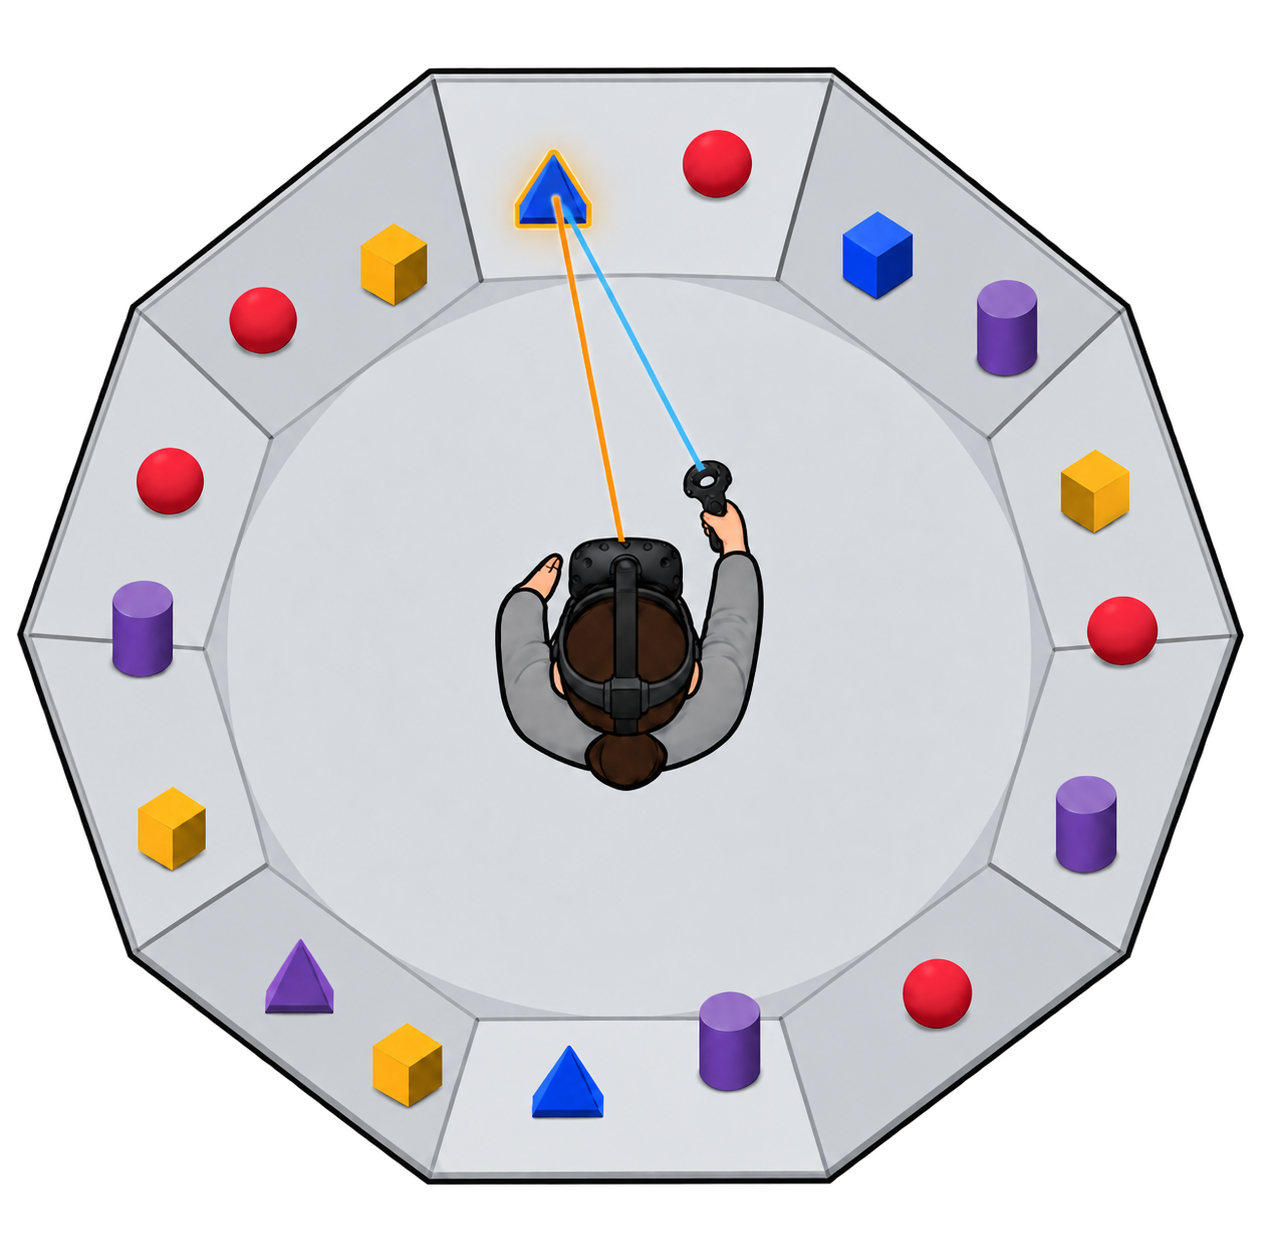
\includegraphics[width=0.6\linewidth]{image.png}
\caption{Top-down view of the search scene. The seated participant is surrounded by wall panels holding colored geometric objects. The gaze ray (orange) and controller ray (blue) converge on the highlighted target, the state in which the participant is ready to select with the trigger. The layout is illustrative; the drawn object count is schematic; object positions and target identity vary by trial.}
\label{fig:scene}
\end{figure}

\subsection{Sensing and Guidance State}
The system continuously collects eye-gaze origin, direction, and validity; head pose; right-controller pose; and ray-object intersections. A local state machine combines these observations with the target geometry to track the participant's progress through the search: turning toward the target wall, refining within the wall, acquiring the target with gaze, pointing with the controller, and becoming ready to select. Additional states cover suspended or paused operation. Each state transition is logged with its cause.

Because guidance is only as reliable as the evidence behind it, the state machine issues new gaze-dependent guidance only when gaze data are valid and recent. Gaze ray hits, gaze-vicinity candidates, and controller hits are treated as separate observations. When gaze-vicinity regions overlap, the closest object is selected. A controller hit immediately suppresses contradictory directional cues, even before the dwell required for spoken pointing confirmation has elapsed, so the system does not direct the participant away from an object they are already pointing at. Gaze confirmation, controller confirmation, and trigger selection are recorded as distinct events.

\subsection{Short-Term Interaction Memory}
To give guidance continuity, the system maintains two short-term memories. A spatial history tracks turning progress and supports cues that return the participant to the target. A speech-decision memory records what the system actually said and how the guidance state changed. Each speech entry stores its relative age, context, and whether playback completed or was interrupted; each state entry stores the prior and current states and the reason for the transition. The speech and transition lists each retain at most four entries; snapshots sent to Jev exclude entries older than 15 seconds. This bounded recent context is related to the context-management motivation of EmBARDiment~\cite{bovo2025embardiment}, but the current implementation does not use its object-admission or dropout policy. The separate spatial history retains up to three seconds or 384 target-relative gaze observations and clears on invalid evidence, source changes, or observation gaps longer than 100~ms. These limits are engineering settings, not validated fixation or blink thresholds. Gaze-vicinity confirmation currently requires 100~ms of valid qualifying evidence; invalid evidence resets its entry timer, and reacquisition after a spoken confirmation requires 150~ms of valid gaze away. Those interaction gates do not admit objects to speech memory, and missing gaze is not counted as observed dwell. The memory is cleared whenever guidance resets and is copied before each asynchronous request. This memory is deliberately scoped to the current task: it does not build a persistent participant profile or attempt to infer unobserved mental states.

\subsection{Agent Decisions and Playback Control}
Jev selects from a constrained set of options rather than generating free-form instructions. Local geometry and state rules first filter the phrase library to candidates that are valid in the current situation. Each request to Jev contains a state snapshot, recent memory, playback status, and two to five eligible phrases. Jev then chooses the wording and whether to speak now or wait. Target definition and geometric reasoning remain local. Eligibility filtering and playback revalidation reduce spatially incorrect or stale guidance, but tracking error, imperfect geometry and software faults can still produce unhelpful instructions; recorded-sequence and headset checks remain necessary.

Because cloud responses arrive asynchronously, the participant's state may change before a decision returns. A local speech scheduler therefore revalidates each decision against the current state, evidence, pacing, and object intersections before playback, and discards decisions that are stale or conflict with the current situation. Feedback that qualifies for local handling is played from prepared phrases without waiting for a new cloud decision, subject to the same checks. Each completed or interrupted utterance updates both the memory and the event log. Model latency, deferral, cancellation, fallback, and playback onset are logged separately, so any delay in speech can be attributed to the stage that caused it.

\begin{figure}[htbp]\centering
\IfFileExists{voice-guidance-memory-architecture.pdf}{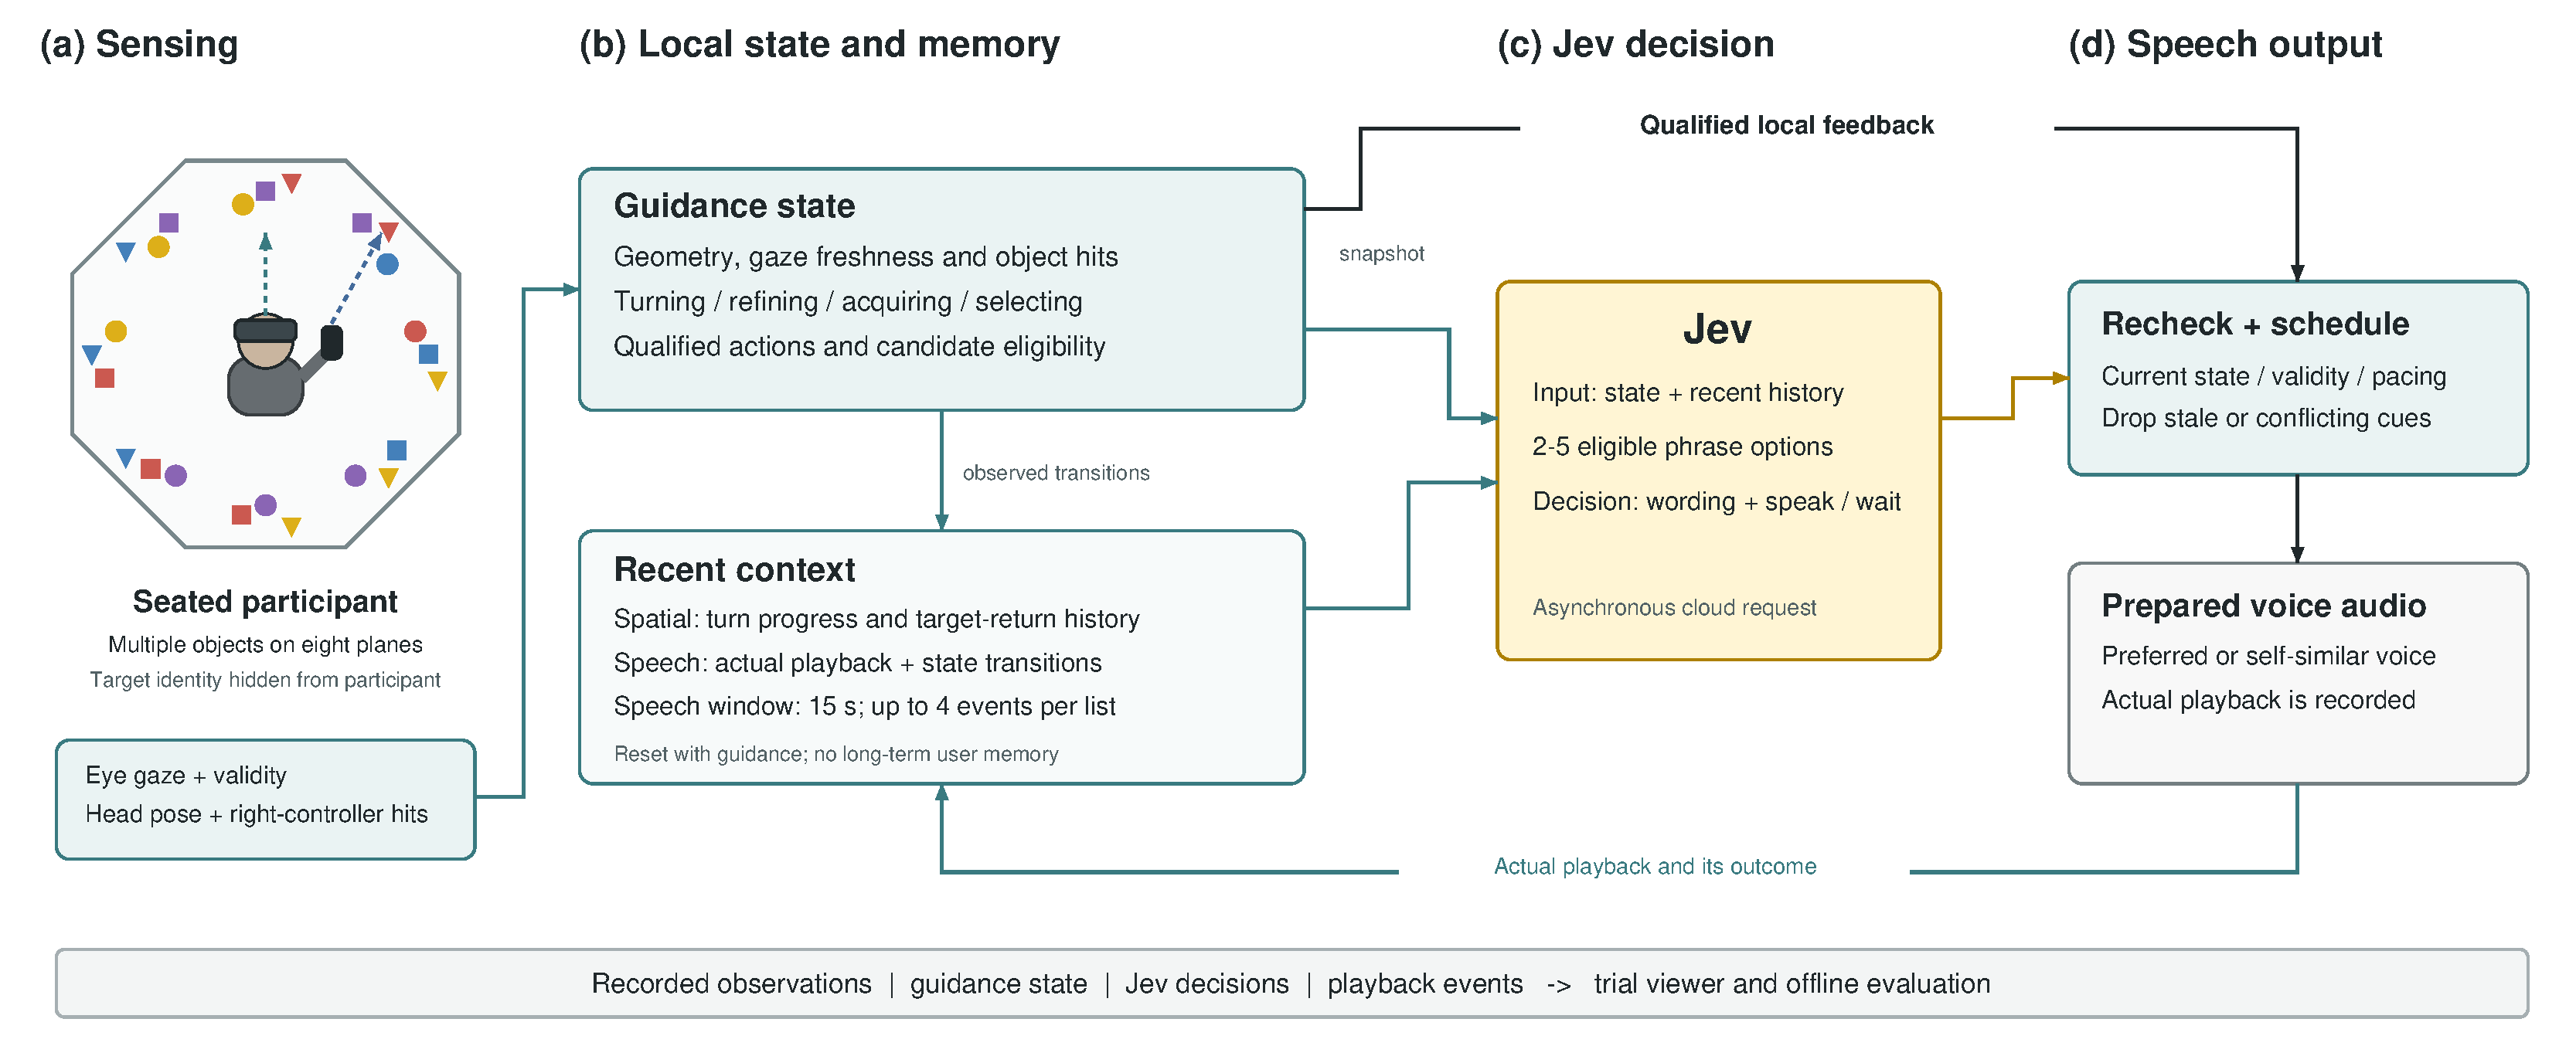
\includegraphics[width=\linewidth]{voice-guidance-memory-architecture.pdf}}{\fbox{\parbox{0.94\linewidth}{Gaze and controller observations $\rightarrow$ local state and bounded context $\rightarrow$ eligible choices for Jev $\rightarrow$ current-state recheck $\rightarrow$ prepared voice playback. Qualified local feedback also enters the recheck stage.}}}
\caption{System architecture. (a) Gaze, head, and controller data are sensed. (b) A local state machine and short-term memory determine which guidance actions are valid. (c) Jev chooses wording and timing from eligible options. (d) The scheduler revalidates each cue against the current state before playback. Actual playback feeds back into memory. The scene inset is schematic and does not reflect stimulus count or any participant-visible target cue.}
\label{fig:architecture}
\end{figure}

\subsection{Voice Preparation and Telemetry}
All voice audio is pre-synthesized with ElevenLabs, which supplies both the catalog voice and the self-similar voice. To support the self-similar condition, each participant records the same standard passage in their usual speaking voice. Both conditions share the semantic phrase library, guidance policy, and playback routing. Voice condition is the intended manipulation; behavior-dependent wording, hint counts and synthesized acoustics need not be identical. The preparation pipeline checks wording and library readiness. Per-voice intelligibility, loudness and acoustic comparability still require pilot verification; automated checks do not establish perceptual equivalence. No pitch or spatial effects are applied to the self-similar voice. We log the provider, model, voice ID, library version, and synthesis settings.

A trial viewer aligns gaze and controller state, guidance transitions, agent decisions, and playback events with trial geometry on a common timeline. Trial-level aggregates are stored separately from the raw gaze, motion, and event streams. Effective gaze sampling rate must be verified from distinct source timestamps on the tested headset build rather than inferred from the nominal specification or application polling rate. Similarly, we report ray intersections as gaze hits and do not label them as fixations unless a validated event classifier is applied.
\section{Experiment}
\subsection{Task}
Participants will perform an agent-guided object-search task while seated on a swivel chair. Multiple colored geometric objects will be scattered across eight surrounding vertical planes. The application will know the target identity, but the participant will not receive a color-and-shape description before searching. Instead, the agent will guide the participant toward the target wall and then refine the direction horizontally, vertically or diagonally. The participant will select an object using the right-controller ray and trigger. Looking at an object, receiving a gaze confirmation or pointing at it will not itself complete the trial.

Each trial will begin with the participant looking at a readiness cross. After readiness is established, an opening directional cue will play while the objects remain hidden. Object reveal will start active search timing. A correct trigger selection will stop timing and produce success feedback; an incorrect selection will be counted and search will continue. This separates readiness and opening guidance from the timed search interval while retaining their timestamps for analysis.

\subsection{Design and trial allocation}
The study will use a within-participant comparison of two voice conditions: a participant-preferred catalog voice and a self-similar synthetic voice. Both conditions will use the same guidance policy, semantic phrase library, selection method and visual-feedback settings. Actual phrase sequences may differ because guidance responds to behavior. The comparison will therefore concern voice identity within an adaptive assistance system; it will not estimate the effect of gaze contingency itself.

A saved, balanced randomized allocation will assign preferred-first or self-similar-first order. Each participant will complete two measured blocks of 40 trials, one per voice, following one practice trial. The practice trial will use the first voice in the assigned order: preferred catalog voice for Order A, or self-similar voice for Order B. Practice will be excluded from measured outcomes. A seed will make the trial and layout schedules reproducible. Nominal horizontal-angle quotas will be identical across blocks; trial order and left/right assignments will be randomized subject to those quotas.

\begin{table}[htbp]\centering
\caption{Study allocation. Nominal wall angles are schedule categories, not exact object bearings or accumulated head rotation.}
\begin{tabularx}{\linewidth}{@{}lX@{}}\toprule
Parameter & Allocation \\\midrule
Voice conditions & Preferred catalog voice; self-similar synthetic voice \\
Measured trials & 40 per block; 80 per participant \\
Practice & One trial; excluded from outcomes \\
Absolute nominal wall angle & Eight trials each at 0, 45, 90, 135 and 180 degrees per block \\
Vertical allocation & 20 targets above and 20 below readiness-cross height per block \\
Condition order & Counterbalanced preferred-first and self-similar-first \\
Selection & Right-controller ray and a trigger press \\\bottomrule
\end{tabularx}
\end{table}

Objects will vary in within-plane position, so the exact starting angle and target height will be recorded in addition to the assigned wall. The vertical allocation will use target-center height relative to the readiness cross, not the participant's seated eye height. Feasible height ranges and realized quotas will be checked in pilot schedules before the study release is frozen.

\begin{figure}[htbp]\centering
\IfFileExists{study-procedure-current.pdf}{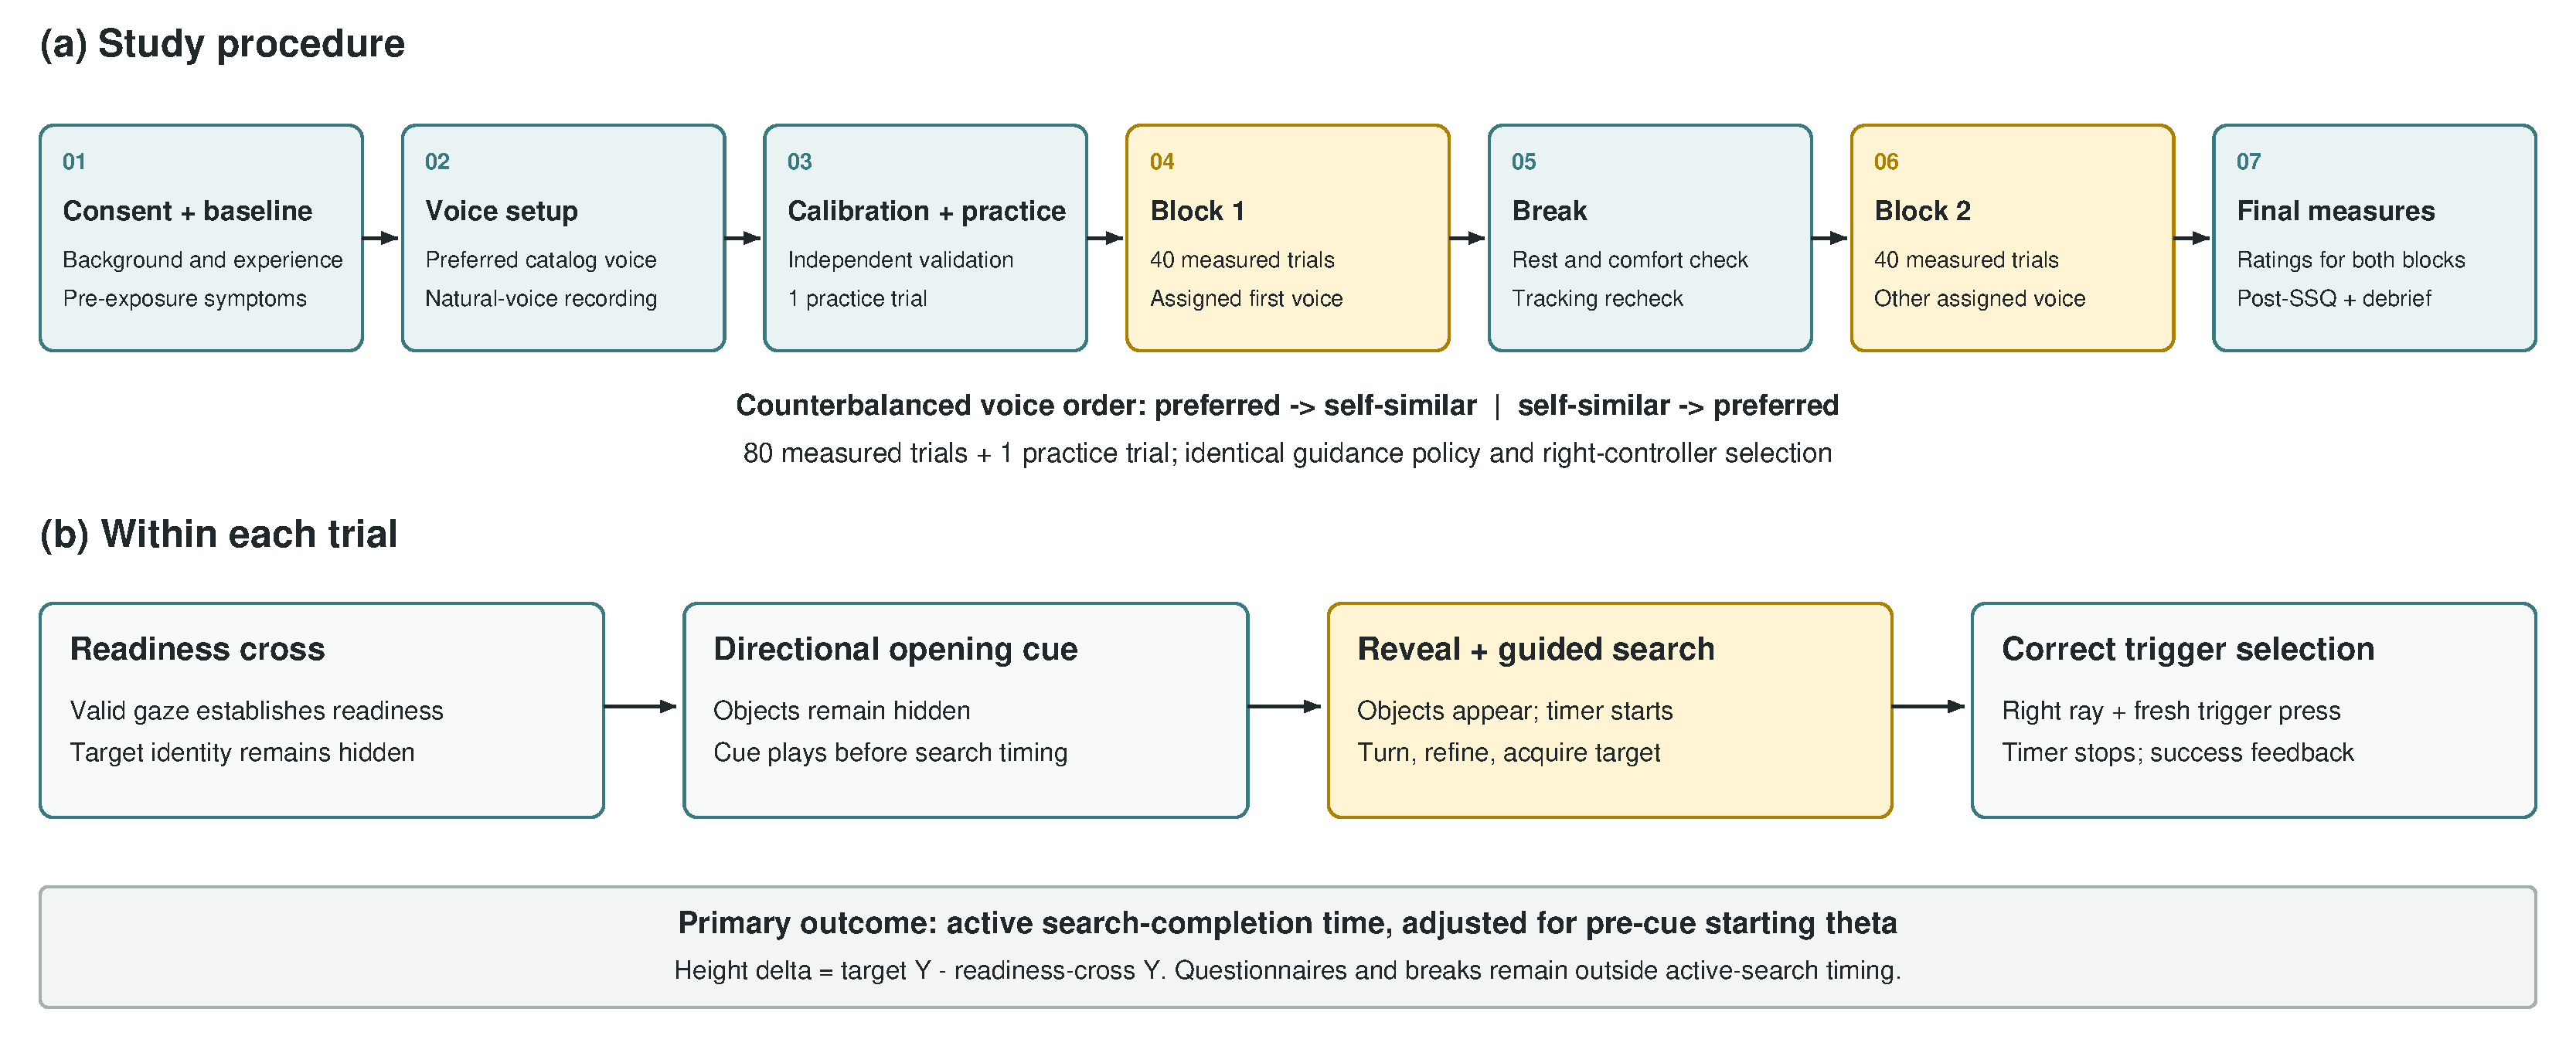
\includegraphics[width=\linewidth]{study-procedure-current.pdf}}{\fbox{\parbox{0.94\linewidth}{Consent and setup $\rightarrow$ calibration and practice $\rightarrow$ 40-trial voice block $\rightarrow$ break $\rightarrow$ 40-trial voice block $\rightarrow$ survey and debrief. Within each trial: readiness cross $\rightarrow$ opening cue $\rightarrow$ object reveal and active search $\rightarrow$ correct trigger selection.}}}
\caption{Study procedure and trial timing. Opening guidance precedes object reveal; active completion time ends at correct right-trigger selection. Questionnaires and between-trial breaks remain outside active-search timing.}
\label{fig:study-procedure}
\end{figure}

\subsection{Measures}
\subsubsection{Task performance}
\paragraph{Active completion time.} The primary outcome will be elapsed active-search time in seconds from object reveal ($t_0$) to the correct right-trigger selection ($t_1$), excluding the union of recorded pause intervals within that interval:
\[
T_{\mathrm{active}}=(t_1-t_0)-T_{\mathrm{paused}}.
\]
Lower values will indicate faster completion. Readiness, opening guidance, post-selection feedback, questionnaires and between-trial breaks will not contribute to this outcome. An unfinished trial will retain its observed exposure and outcome, but will not receive a successful completion time. The full interval from opening-cue onset to selection will be retained separately to describe the complete instructed task duration.

\paragraph{Target contact and selection errors.} Time to first target gaze will be the active-clock time of the first valid, recorded gaze-ray intersection with the target. Time to first controller contact will use the first tracked right-controller ray--target intersection. Time to final target gaze will denote the last observed valid target intersection during the trial, not a fixation duration or a spoken confirmation. These event times will remain distinct from trigger selection and from the larger gaze-vicinity region used by the guidance system. Incorrect selections will be counted as trigger selections of non-target objects. If no valid target contact is observed, its latency will remain missing rather than being set to zero. Contact times will retain their source and sampling resolution.

\subsubsection{Starting geometry and search behavior}
\paragraph{Starting angle, height and distance.} Before the opening cue, the system will record the reference origin, readiness-cross position and target position. Starting theta ($\theta_0$) will be the signed angle about world up between the horizontal origin-to-cross and origin-to-target vectors. Its magnitude $|\theta_0|$ will quantify horizontal turn demand, and its sign will preserve direction. Degenerate horizontal vectors will be marked unavailable. The primary analysis will adjust for $|\theta_0|$ rather than divide completion time by degrees. Nominal wall-angle assignment, exact pre-cue theta, and head-to-target error observed after reveal will remain separate variables.

Signed target-height difference will be $\Delta h=y_{\mathrm{target}}-y_{\mathrm{cross}}$, in metres; positive values will indicate above-cross targets. Euclidean target distance will be the three-dimensional distance between target center and the first valid tracked head position after reveal, with that observation's timestamp retained. This post-reveal distance will not substitute for a missing pre-cue geometry snapshot. All positions used in a calculation will share a recorded coordinate frame.

\paragraph{Head movement and zone coverage.} Gross head translation will sum distances between adjacent valid head positions, in metres. Gross head rotation will sum shortest quaternion angular displacements between adjacent valid orientations, in degrees. Fixed-axis component totals will be retained separately and will not be mislabeled as Euler yaw, pitch and roll. Invalid intervals, pauses and excessive sample gaps will break accumulation rather than be interpolated across; covered time and gap counts will accompany totals. These measures describe head movement, not independently tracked chair rotation.

Distinct walls visited, wall transitions and revisits will summarize search coverage using stable valid gaze observations and a versioned zone-assignment rule. Transitions across tracking gaps will not be inferred. More motion or more visits will not by themselves establish worse strategy, since geometry and available observations also affect these totals.

\paragraph{Instructions and guidance timing.} Instruction count will include guidance utterances whose playback actually starts during active search, including delivered repeats. Requested repeats, delivered repeats and interrupted utterances will be retained separately; model requests, prefetched audio and success speech will not be counted as delivered search instructions. Opening cues and success feedback will retain separate event labels. Timing analysis will distinguish evidence qualification, decision-request latency, model deferral, scheduling delay and audio onset. Gaze confirmations and controller confirmations will be evaluated separately against their corresponding evidence.

\subsubsection{Subjective measures}
\paragraph{Workload.} Six NASA-TLX dimensions---mental, physical and temporal demand, performance, effort and frustration---will be rated separately for each voice block during the final survey, after both blocks. The study will use a documented 0--10 adaptation, without pairwise weighting. Performance will run from Perfect to Failure; other dimensions will run from Very low to Very high. Individual ratings and the unweighted mean of all six completed dimensions will be retained; higher scores will indicate greater workload or poorer perceived performance. The source instrument is \href{https://doi.org/10.1016/S0166-4115(08)62386-9}{Hart and Staveland's NASA-TLX}.

\paragraph{Motivation and activity experience.} The \href{https://selfdeterminationtheory.org/intrinsic-motivation-inventory/}{Intrinsic Motivation Inventory} will contribute interest/enjoyment (7 items), effort/importance (5), pressure/tension (5), and value/usefulness (7). Responses will range from 1 = Not at all true to 7 = Very true. Published reverse keys will be applied before averaging each complete subscale. Interest/enjoyment will represent intrinsic motivation; the four subscales will not be combined into an overall IMI score. Activity wording will refer to the completed search block, with task-specific adaptations documented.

\paragraph{Agent perception.} Twenty-one items from \href{https://doi.org/10.1145/3651288}{Guo et al. (2024), Appendix A, Table A1} will assess co-presence (Q1--6), perceived intelligence (Q13--18), appealing/eerie/familiar impressions (Q20--22), and perceived anthropomorphism (Q37--42). ``Virtual character'' will be adapted to ``voice agent.'' Responses will range from 1 = Very strongly disagree to 7 = Very strongly agree. The three six-item constructs will have separate complete-scale means. Q20--22 will be analyzed individually, without a combined eeriness score. These attributed qualities will not be interpreted as actual agent intelligence or sentience.

\paragraph{Voice experience and reliance.} Twelve custom 1--7 agreement items will assess voice similarity, responsiveness, helpfulness, distraction, familiarity, trust, comfort, uncanniness, reliance, naturalness, willingness to follow and motivation to act without guidance. Voice similarity will serve as a manipulation check. Voice liking and retrospective percentage of guidance use will each use 0--100 responses with separate unable-to-answer options. These 14 numeric items will be analyzed separately; they are not a validated composite scale. Liking during voice audition will remain separate from condition-specific liking collected at the end.

\paragraph{Symptoms and debrief.} The 16 \href{https://doi.org/10.1207/s15327108ijap0303_3}{Simulator Sickness Questionnaire} symptoms will be rated from 0 = None to 3 = Severe before headset exposure and after headset removal. Canonical total or subscale scores will require the published membership and weights. Open debrief questions will explore perceived performance, guidance experience, own-voice comfort, possible use cases and voice preference; broad experience questions will precede specific eeriness or inner-dialogue probes.

Each condition-specific set in the final survey will therefore contain 65 numeric responses (130 across both sets): six workload ratings, 24 IMI items, 21 Guo items and 14 custom ratings. Technical checks and optional text will be additional. Questionnaire observations will have participant-by-block scope even when copied into per-trial summary files; they will not be treated as 40 independent responses. Missing answers will not be replaced with zero.

\subsubsection{Measurement quality}
Tracking validity, observation age, data coverage, gaps and spatial-validation error will accompany gaze-derived measures. Ray intersections and vicinity hits will not be labeled fixations, and render-frame observations will not establish native eye-tracker sampling frequency. Pupil-based workload inference and fixation/saccade outcomes will require independent validation before inclusion. Trial performance and subjective summaries will remain linked to separate raw gaze, motion and event records through participant, session, block and trial identifiers. Scale metadata will distinguish the present 0--10 workload form from any earlier exports using another range.

\subsection{Research questions}
The primary question will be whether self-similar and preferred catalog voices differ in active completion time after accounting for absolute starting theta. Secondary questions will concern workload and the four IMI subscales. Exploratory questions will concern agent perception, eeriness, voice experience, reliance, search behavior and variation in the voice contrast with starting angle. The primary voice contrast will be two-sided; a directional benefit of self-similarity will not be assumed. Repeated trials will not be treated as independent participants.

\subsection{Participants}
Participants will be consenting adults able to understand the task, hear the guidance, view the scene with usual correction and safely use the seated setup and right controller. Handedness, visual correction and prior XR and voice-assistant experience will be recorded. Recruitment size and the enrollment ceiling will be determined before recruitment using power analysis for the theta-adjusted repeated-measures outcome, including plausible within-participant variation and incomplete observations.

\subsection{Procedure}
After consent, participants will complete background questions and baseline symptom ratings. They will choose a preferred catalog voice, rate auditioned voices, record a standard passage in their natural voice for synthesis, and confirm comfortable, clear audio for each condition. Preferred gender presentation will be chosen explicitly rather than inferred from participant gender.

The researcher will fit the headset and conduct vendor calibration followed by independent spatial validation across relevant heights, wall boundaries, distances and head orientations. Validation targets will be separate from any targets used to fit an offset correction. Standardized instructions will explain that participants will rely on the agent to discover the target and use the right trigger to select it. Participants will then complete the single practice trial and the two assigned 40-trial blocks.

No questionnaire will interrupt the block sequence. During the final survey, the same condition-specific questionnaire will be completed twice, once referring to Block 1 and once to Block 2, with identical item wording and order. Breaks will be offered between trials and at the block boundary; any necessary in-trial pause will be logged immediately. Tracking will be rechecked between blocks and after headset adjustment. After headset removal, participants will first complete the final symptom check, then the two retrospective condition-specific sets, comparative voice preference and debrief. Participants may request a pause or stop, and symptoms or technical problems will prompt researcher assessment.

\subsection{Pilot testing and parameter checks}
Before confirmatory recruitment, pilot sessions will verify the realized angle/height schedules, target visibility and seated comfort, readiness and selection behavior, gaze validity, audio timing and wording, and reconstruction of trial events from the saved data. Survey comprehension and completion time will also be measured. Calibration acceptance, practice proficiency, timeout and technical-stop criteria will be set from those checks and recorded with the study build and questionnaire versions. Pilot observations will be reported as such rather than presented as study outcomes or evidence for a voice-condition effect.

\section{Planned Analysis}
\subsection{Primary contrast}
The primary estimand will compare active completion time under the self-similar and participant-preferred catalog voices, standardized to the same starting-difficulty distribution. A trial-level mixed-effects analysis of log completion time will account for participant clustering, voice condition, period/order, trial progression and absolute pre-cue starting theta. Report the voice time ratio and uncertainty using a two-sided contrast.

A prespecified low-complexity function of theta will allow nonlinearity; nominal-angle strata will support balance plots and a categorical sensitivity analysis. Zero-degree trials will remain in the analysis, and completion time will not be divided by angle. The model's random-effects structure, angle function and smallest meaningful effect will be finalized with simulation before confirmatory recruitment. Participant count will be justified under that same model; repeated trials will not be treated as independent participants.

\subsection{Secondary and exploratory outcomes}
Retrospective condition-specific ratings will be collected only after both blocks, with actual survey timestamps retained. Reference scope remains participant-by-block. Recall and recency effects will be considered when interpreting condition differences; these are not immediate post-block measurements. Individual workload dimensions and complete unweighted workload means will be summarized by participant and block. IMI subscales and the three six-item agent-perception constructs will remain separate scores. The additional Guo Q20--22 appealing, eerie and familiar ratings will be analyzed individually, without a combined eeriness score. Voice similarity will be a manipulation check. Custom experience ratings and self-reported guidance use will be analyzed individually. Multiplicity families and secondary contrasts will be specified before confirmatory analysis.

Instruction count, observed gaze path and other behavior potentially caused by voice condition will not automatically be covariates in the primary model. Voice-by-theta variation, selected catalog voice, acoustic quality and guidance timing will be exploratory or sensitivity analyses with their assumptions reported.

\subsection{Incomplete and interrupted observations}
Raw attempts, incorrect selections, pause intervals, timeouts, technical failures and withdrawals will be retained. Stopped trials will not be coded as successful completion times. Timeout/censoring rules and the missing-data estimand will be specified before collection; slow trials will not be removed solely for being slow. Missing responses will not be replaced with zero. Questionnaire scores will follow the complete-subscale rule, with item-level missingness reported. Disliking or failing to recognize a cloned voice will not by itself exclude a participant.

\subsection{Guidance and qualitative evaluation}
Engineering analysis will distinguish event qualification, decision latency, model deferral, scheduling delay and actual playback. Gaze and controller confirmation will be evaluated separately. Sequence-level review will include what happened before and after a cue. Automatic checks and model-judge ratings will remain advisory engineering evidence, not participant perception scores.

Debrief responses will be coded with a documented thematic process and an audit trail, with independent review of a subset. Perceived performance, voice comfort, reliance and possible own-voice use cases will be interpreted alongside, but not substituted for, measured task performance.
\section{Contributions and Limitations}
The study will connect a personalized voice comparison to a measurable gaze-guided search task. Its system combines locally verified spatial evidence, bounded interaction history, constrained language-model decisions and recorded playback. Separating these stages permits analysis of whether a poor cue arose from sensing, state qualification, model choice, scheduling or audio delivery.

The comparison does not isolate gaze contingency, memory or a standalone language-model effect because those components are shared across voices. Preferred catalog voices introduce deliberate personalization and voice heterogeneity. Self-similar synthesis quality, recognition and naturalness may vary across participants and will be recorded.

The selected agent-perception measures originate in an embodied-collaborator context and are adapted to a voice-only agent. Participant attributions do not establish actual emotions, intelligence or sentience. The final questionnaire battery will contain 130 condition-specific numeric ratings across two retrospective sets, plus symptoms, technical checks and debrief. Its burden and ability to distinguish the two blocks will be checked during pilots. Delayed administration may introduce recall and recency effects; findings will not be described as immediate post-block ratings. Gaze sampling quality and spatial accuracy must be established on the study headset; interaction proxies alone do not establish fixations or workload.

The seated geometry, right-controller interaction and hidden-target task limit generalization to free walking or tasks where target identity is known in advance. Cloud dependencies and voice-library versions can affect reproducibility, so the research release and configuration will be pinned and changes documented. Consent and data handling will describe the services actually used and the identifiability of recorded or synthesized voices.
\section{Conclusion}
Follow My Voice will test whether self-similar and participant-preferred catalog voices produce different performance and experiences during seated, gaze-guided mixed-reality search. Both conditions will share a stateful guidance policy and right-controller selection. Completion time will be analyzed with starting-theta adjustment, while workload, motivation and agent/voice perceptions will provide complementary outcomes. The study will preserve the distinction between sensed evidence, model decisions, actual speech and participant interpretations.
\bibliographystyle{plain}
\bibliography{references}
\end{document}
